\documentclass[a4paper, 12pt]{article}

\usepackage[english,russian]{babel}
\usepackage[T2A]{fontenc}
\usepackage[utf8]{inputenc}
\usepackage{geometry}
\usepackage{enumitem}
\usepackage{setspace}
\usepackage{amssymb}
\usepackage{graphicx}
\usepackage{wrapfig}
\usepackage{float}
\usepackage{amsmath}
\usepackage{textcomp}
\usepackage{dsfont}

\geometry{top=5mm, left=1cm}
%\setlength{\parindent}{0}
\renewcommand{\arraystretch}{1.2}
\linespread{1}

\begin{document}
    \begin{center}
        \textbf{Сферическая геометрия тест №4}\\
        Расстояние между точками, углы между прямыми, сферические окружности.
    \end{center}

    \begin{center}
        \textbf{№ 1}
    \end{center}

    На сфере радиуса 7 см построена сферическая окружность радиусом 3 см.
    Чему равен радиус малой окружности, совпадающей с данной?

    \textbf{Решение}\\

    \begin{center}
        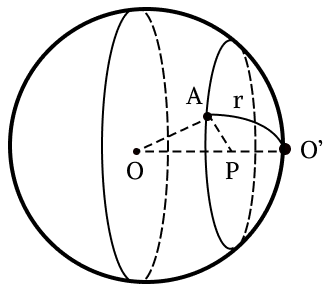
\includegraphics[width=0.2\textwidth]{images/img1}\\
    \end{center}

    1) $OO' = OA = 7$ см, $AP \bot OO'$

    2)
    \[
        r = 7*\angle O'OA \rightarrow \angle O'OA = \frac{3}{7} \text{ см}
    \]

    3)
    \[
        AP = OA * \sin POA = 7 * \sin \frac{3}{7} \text{ см}
    \]

    Ответ: $7\sin \frac{3}{7}$ см

    \begin{center}
        \textbf{№ 2}
    \end{center}

    Проведены две сферические прямые, пересекающиеся под углом $\alpha$,
    перпендикулярно к ним проведена третья сферическая прямая.
    Чему равен угол $\alpha$, если сферическое расстояние между точками пересечения
    двух прямых третьей равно $h$, а радиус сферы равен $R$?

    \textbf{Решение}\\

    \begin{center}
        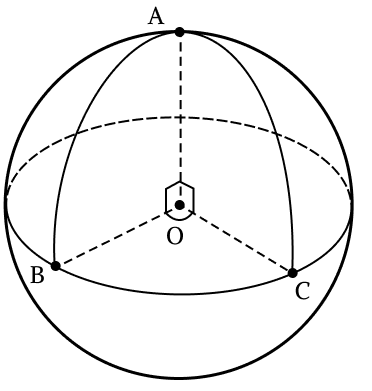
\includegraphics[width=0.2\textwidth]{images/img2}\\
    \end{center}

    \[
        BC = h = \alpha R \rightarrow \alpha = \frac{h}{R}
    \]

    Ответ: $\frac{h}{R}$

\end{document}
